\begin{center}
    \section{Validaci\'on del modelo}
\end{center}

\noindent
\justify

Para la validaci\'on del modelo CFD-DEM desarrollado, se aplic\'o el modelo para resolver el problema de Fessler & Eaton$^{\cite{Fessler1999}}$, en donde se investig\'o el efecto de la turbulencia generada por part\'iculas de cobre de $70 [\mu m]$ de di\'ametro sobre un flujo \textit{orientado hacia atr\'as}, como se muestra en la Figura \ref{problemaVal}.

\begin{figure}[h!]
    \centering
    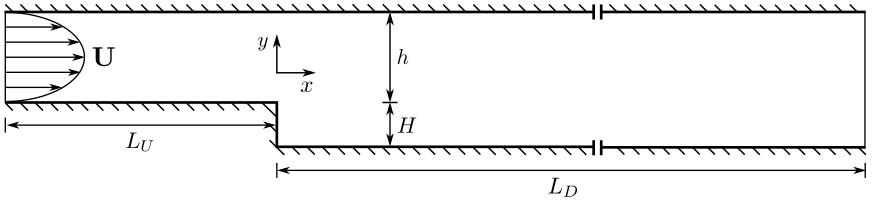
\includegraphics[width=\textwidth]{Images/Fessler.PNG}
    \caption{Geometr\'ia de estudio.}
    \label{problemaVal}
\end{figure}

\subsection{Descripci\'on del problema}

\noindent
\justify

En 1999, Fessler & Eaton estudiaron el efecto de part\'iculas de vidrio y cobre de distintos tama\~nos ($70$, $90$ y $150 [\mu m]$ de di\'ametro), a diferentes cargas m\'asicas (entre el 3 y el 40 \% del flujo m\'asico) y a las mismas condiciones experimentales de velocidad y presi\'on en donde se apreci\'o una atenuaci\'on del flujo relacionada con un decaimiento en el n\'umero de Stokes de las part\'iculas.

\noindent
\justify

La motivaci\'on de esta investigaci\'on recae en la complejidad de las interacciones entre part\'iculas peque\~nas y densas con la fase turbulenta de una sustancia gaseosa; adem\'as de la importancia en diferentes casos, de car\'acter industrial y natural, en donde se producen flujos particulados que son, muchas veces, inentendidos. En pocos aspectos, tales como la dispersi\'on de part\'iculas en flujos homog\'eneos, se pueden llevar a cabo estudios anal\'iticos con altos niveles de precisi\'on. Sin embargo, la mayor\'ia de los casos en la realidad comprenden flujos heterog\'eneos y anisotr\'opicos sujetos a inestabilidades con marcadas variaciones entre flujo y flujo. 

\noindent
\justify

Se ha reportado en la literatura que los niveles de turbulencia pueden ser moderados con la ayuda de la carga de diferentes masas. Investigaciones como la de Hetsroni$^{\cite{Hetsroni1989}}$ y Gore & Crowe$^{\cite{Gore1991}}$ establecieron los cimientos del comportamiento turbulento en la interacci\'on fluido - part\'icula. 